\section{eo\-Gnuplot1DSnapshot Class Reference}
\label{classeo_gnuplot1_d_snapshot}\index{eoGnuplot1DSnapshot@{eoGnuplot1DSnapshot}}
Plot stats through gnuplot.  


{\tt \#include $<$eo\-Gnuplot1DSnapshot.h$>$}

Inheritance diagram for eo\-Gnuplot1DSnapshot::\begin{figure}[H]
\begin{center}
\leavevmode
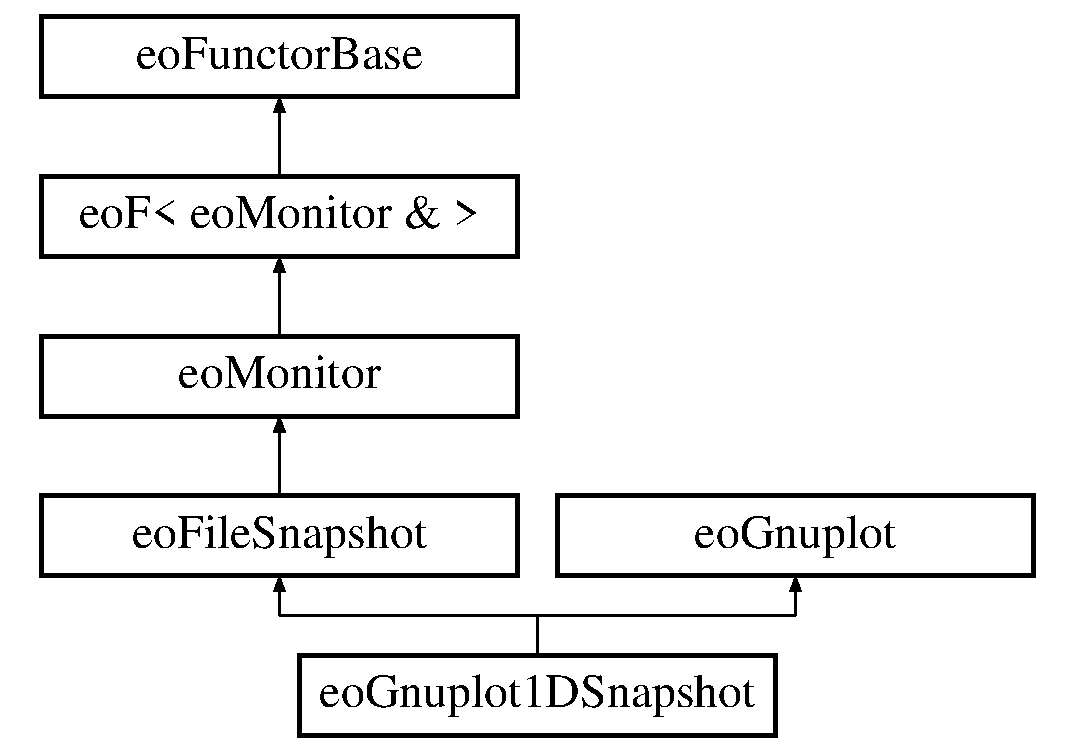
\includegraphics[height=5cm]{classeo_gnuplot1_d_snapshot}
\end{center}
\end{figure}
\subsection*{Public Member Functions}
\begin{CompactItemize}
\item 
{\bf eo\-Gnuplot1DSnapshot} (std::string \_\-dirname, unsigned \_\-frequency=1, std::string \_\-filename=\char`\"{}gen\char`\"{}, std::string \_\-delim=\char`\"{} \char`\"{}, unsigned \_\-counter=0, bool \_\-rm\-Files=true)\label{classeo_gnuplot1_d_snapshot_a0}

\item 
{\bf eo\-Gnuplot1DSnapshot} (std::string \_\-dirname, {\bf eo\-Real\-Vector\-Bounds} \&\_\-bounds, unsigned \_\-frequency=1, std::string \_\-filename=\char`\"{}gen\char`\"{}, std::string \_\-delim=\char`\"{} \char`\"{}, unsigned \_\-counter=0, bool \_\-rm\-Files=true)\label{classeo_gnuplot1_d_snapshot_a1}

\item 
{\bf eo\-Gnuplot1DSnapshot} ({\bf eo\-File\-Snapshot} \&\_\-f\-Snapshot)\label{classeo_gnuplot1_d_snapshot_a2}

\item 
{\bf eo\-Gnuplot1DSnapshot} ({\bf eo\-File\-Snapshot} \&\_\-f\-Snapshot, {\bf eo\-Real\-Vector\-Bounds} \&\_\-bounds)\label{classeo_gnuplot1_d_snapshot_a3}

\item 
virtual {\bf eo\-Monitor} \& {\bf operator()} ()\label{classeo_gnuplot1_d_snapshot_a5}

\begin{CompactList}\small\item\em The operator(void): opens the std::ostream and calls the write method. \item\end{CompactList}\item 
virtual std::string {\bf class\-Name} () const \label{classeo_gnuplot1_d_snapshot_a6}

\begin{CompactList}\small\item\em Class name. \item\end{CompactList}\item 
virtual void {\bf handle\-Bounds} ({\bf eo\-Real\-Vector\-Bounds} \&\_\-bounds)\label{classeo_gnuplot1_d_snapshot_a7}

\item 
void {\bf set\-Point\-Size} (unsigned \_\-point\-Size)\label{classeo_gnuplot1_d_snapshot_a8}

\end{CompactItemize}
\subsection*{Protected Attributes}
\begin{CompactItemize}
\item 
unsigned {\bf point\-Size}\label{classeo_gnuplot1_d_snapshot_p0}

\end{CompactItemize}


\subsection{Detailed Description}
Plot stats through gnuplot. 

\begin{Desc}
\item[Author:]Marc Schoenauer 2000 \end{Desc}
\begin{Desc}
\item[Version:]0.0\end{Desc}
This class plots through gnuplot the {\bf eo\-Stat}{\rm (p.\,\pageref{classeo_stat})} given as argument

Assumes that the same file is re-written every so and so, and plots it from scratch everytime it's called 



Definition at line 51 of file eo\-Gnuplot1DSnapshot.h.

The documentation for this class was generated from the following files:\begin{CompactItemize}
\item 
eo\-Gnuplot1DSnapshot.h\item 
eo\-Gnuplot1DSnapshot.cpp\end{CompactItemize}
